\scanpage{33}
\noindent\begin{tabular}{@{}l|l@{}}
I\uline{ntroduction} vider & Bibliographie mixte.\\
 & mention de C.T.
\end{tabular}

\begin{center}
INSTITUT\\
DES HAUTES ÉTUDES SCIENTIFIQUES\\
\rule{2.3em}{0.4pt}
\end{center}

\uline{Artin}\qquad SGA 4

réf \quad X \quad [1]

X \qquad p.7 \qquad Début de phrase manque

\noindent\rule{\linewidth}{0.4pt}

$\underline{\overline{\mathrm{X}}\mathrm{I}\overline{\mathrm{I}}}$\qquad compléter réf : Giraud

5.10. \qquad \unsure{Compléter|compléter} remarque par réf.\\
\hspace*{5em}aux travaux récents d'Artin

{\color{red!75!black}
\noindent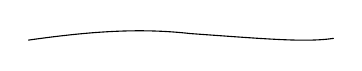
\begin{tikzpicture}[x=\linewidth,y=1ex,baseline=0pt]
\draw[line width=.4pt] (0,0) .. controls (.07,.8) and (.12,1) .. (.17,.55)
 .. controls (.25,.1) and (.29,-.2) .. (.32,.15);
\end{tikzpicture}

$\underline{\overline{\mathrm{IX}}}$\qquad p\unsure{.}\,34 \qquad \unsure{réf|ref} th. de Tsen
}

\noindent\rule{.6\linewidth}{0.4pt}

$\underline{\overline{\mathrm{XIII}}}$\qquad \deleted{p.\unsure{13}} 3.1. \qquad Supposer $X$ noethérien\\
\hspace*{7em}(sinon, p.13 l.$-3$ pas clair)

{\color{gray!80!black}
\noindent\rule{.42\linewidth}{0.4pt}

XIX \qquad p 3,4,10 \qquad p 7 \deleted{\unsure{14|24}},\unsure{18|10},55,39,43
}
% archive sheet number: 32

